\chapter{Design}
This chapter contains the design choices and an explanation of the different design blocks.

\section{CDU}
This section contains the CDU design blocks.
\subsection{Power Supply}
tbw
%The power supply is in charge of providing the system with 3.3 volts. This supply is for analog parts of the CDU and the µ-controller. The design is shown in figure \ref{fig:cdupowersupply}.
%
%\begin{figure}[H]
%\centering
%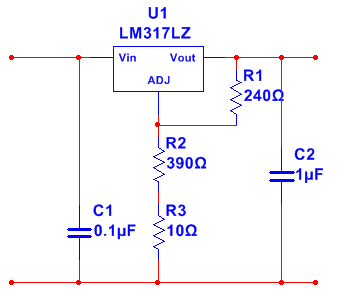
\includegraphics[scale=1]{billeder/cdupowersupply}
%\label{fig:cdupowersupply}
%\caption{CDU Power Supply}
%\end{figure}

\subsection{Sensor Power Supply}
tbw
%\begin{figure}[H]
%\centering
%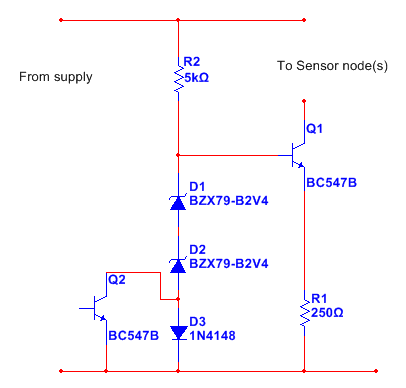
\includegraphics[scale=1]{billeder/cdusensorpowersupply}
%\label{fig:cdusensorpowersupply}
%\caption{Sensor Power Supply part of the CDU}
%\end{figure}

\subsection{Sensor communication}
tbw
%
%\begin{figure}[H]
%\centering
%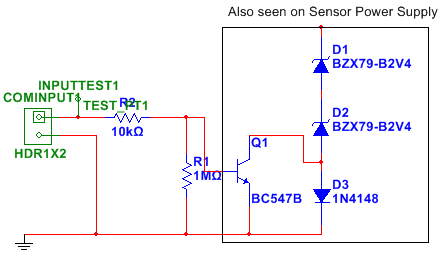
\includegraphics[scale=1]{billeder/cdusensorsend}
%\label{fig:cdusensorsend}
%\caption{Writing to Sensor node(s)}
%\end{figure}

%\begin{figure}[H]
%\centering
%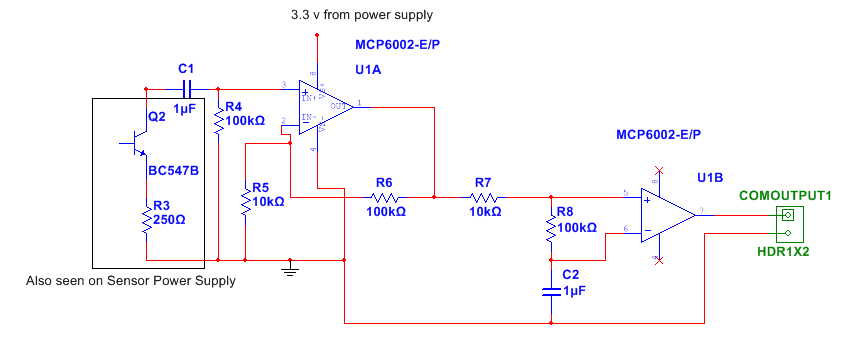
\includegraphics[width=1\textwidth]{billeder/cdusensorread}
%\label{fig:cdusensorread}
%\caption{Reading from Sensor node(s)}
%\end{figure}



\subsection{µ-Controller}
The microcontroller block is a hybrid hardware and software block. Both blocks will be explained in this subsection.
\subsubsection{Hardware}

\subsubsection{Software}
The software on the microcontroller governs the sensor communication, the PC communication and the memory. The hierarchy of software can be seen on the class diagram in figure ~\ref{fig:cduclassd}.

\begin{figure}[H]
\centering
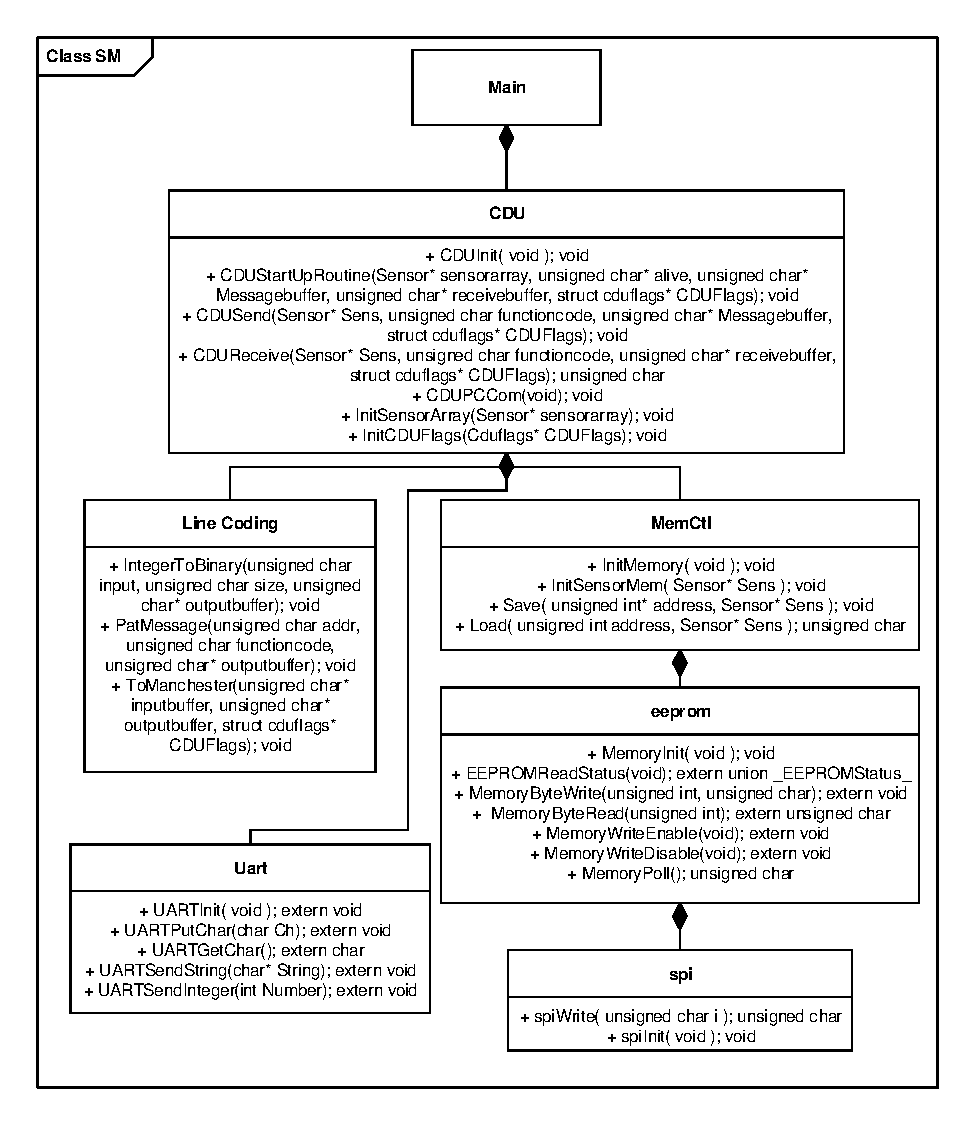
\includegraphics[scale=0.8]{billeder/CDUClassDiagramme}
\label{fig:cduclassd}
\caption{CDU Class diagram}
\end{figure}

\textbf{Variables:}\\
The global variables in the CDU includes 2 structs. These 2 structs will be shown in their own table.
\begin{table}[H]
\begin{tabular}{|l|p{10cm}|}
\hline
\cellcolor[gray]{0.8}\textbf{Variable} &\cellcolor[gray]{0.8} \textbf{Description}\\ \hline
\texttt{comflag} & This varible(flag) determines whether a message is written on the bus.\\ 
\hline
\texttt{msgflag} & This varible(flag) determines whether a message is ready to be written on the bus.\\ 
\hline
\texttt{clk$\_$flag} & This varible(flag) determines whether to put a low or high out on the bus while not communicating.\\ 
\hline
\texttt{recvflag} & This varible(flag) determines whether a message has been received on the bus.\\ 
\hline
\texttt{enableflag} & This varible(flag) determines when a transmission can be written on the bus.\\ 
\hline
\end{tabular}
\label{tab:structcduflags}
\caption{Struct CDUFlags}
\end{table}

\begin{table}[H]
\begin{tabular}{|l|p{10cm}|}
\hline
\cellcolor[gray]{0.8}\textbf{Variable} &\cellcolor[gray]{0.8} \textbf{Description}\\ \hline
\texttt{Address} & This variable contains the address of the sensor node.\\ 
\hline
\texttt{Data} & This variable contains the data of the sensor node.\\ 
\hline
\texttt{Year} & This variable contains the current year.\\ 
\hline
\texttt{Day} & This variable contains the current day.\\ 
\hline
\texttt{Hour} & This variable contains the current hour.\\ 
\hline
\texttt{Minute} & This variable contains the current minute.\\ 
\hline
\texttt{Errors} & This variable contains the errors explained in the protocol section of the architecture document.\\ 
\hline
\texttt{Type} & This variable contains the type of the sensor node.\\ 
\hline
\end{tabular}
\label{tab:structsensor}
\caption{Struct Sensor}
\end{table}

\begin{table}[H]
\begin{tabular}{|l|p{10cm}|}
\hline
\cellcolor[gray]{0.8}\textbf{Variable} &\cellcolor[gray]{0.8} \textbf{Description}\\ \hline
\texttt{message} & The array will contain messages the are to be written to the bus.\\ 
\hline
\texttt{response} & The array will contain messages that have been read from the bus.\\ 
\hline
\texttt{alive} & The array contains values depending if a sensor is alive or not.\\ 
\hline
\texttt{loopcounter} & This variable(counter) is used for writing to the bus.\\ 
\hline
\texttt{recvcounter} & This variable(counter) is used for reading from the bus.\\ 
\hline
\texttt{waitclock} & This variable(counter) is used for delaying when in between writing to the bus and reading from the bus.\\ 
\hline
\texttt{maincounter} & This variable(counter) is used for delaying in between transmission sequences.\\ 
\hline
\end{tabular}
\label{tab:globalvar}
\caption{Global variables}
\end{table}


\textbf{Function descriptions:}\\

\begin{table}[H]
\begin{tabular}{l p{12.5cm}}
\multicolumn{2}{l}{\texttt{\textcolor{blue}{void} CDUInit( \texttt{\textcolor{blue}{void}})}} \\
\hline
Description:& The function is used to Initiate the whole CDU. The proper register settings for timer, uart and spi are set. Arrays and structs are initialised.\\
Parameters:&none\\
Return value:&none\\
\end{tabular}
\end{table}


\subsection{PC communication}
tbw

\subsection{Memory}
tbw

\section{Sensor node}
This section contains the Sensor node design blocks.
\subsection{Communication}
tbw

\subsection{Logic handler}
tbw

\subsection{Power supply}
tbw

\subsection{Sensor}
tbw